\section{Vapour and Humidity}


%Evaporation of Liquids



%Relative Humidity (hygrometer)

\subsection{Measuring Humidity with a Hygrometer}

\subsubsection*{Learning Objectives}
\begin{itemize}
\item{To measure relative humidity}
\item{To explain relative humidity}
\end{itemize}

\subsubsection*{Background Information}
Humidity is the concentration of water vapour present in the air.  We measure humidity by using a hygrometer, which measures the difference in humidity between two thermometers, one of which is in open air and one of which is being cooled by evaporation.  If air contains a lot of vapour, wet objects do not evaporate much.  However, if the air is dry, wet objects evaporate a lot.  By using the evaporation of water from a thermometer, we can measure the amount of vapour in the air.

\subsubsection*{Materials}
Two mercury or alcohol thermometers, container of water, piece of cotton cloth, thread

\subsubsection*{Hazards and Safety}
\begin{itemize}
\item{Be careful when spinning the thermometers over your head.  The thread needs to be strong so that the thermometers do not fly off.  Also, be sure that the area around you is clear so that the thermometers don't hit anything.}
\end{itemize}

\subsubsection*{Preparation Procedure}
\begin{enumerate}
\item{Collect two thermometers.  These are necessary and can be found in any laboratory or hospital supply shop.}
\item{Find a small piece of cotton cloth and a small container of any kind.}
\end{enumerate}

\begin{figure}
\begin{center}
%\def\svgwidth{100pt}
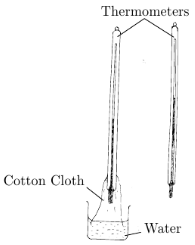
\includegraphics{./img/hygrometer.png}
\caption{A hygrometer for measuring humidity}
\label{fig:hygrometer}
\end{center}
\end{figure}

\subsubsection*{Activity Procedure}
\begin{enumerate}
\item{Pour some water into the container.}
\item{Wrap the bulb of one of the thermometers with the cotton cloth.}
\item{Tie the cloth with thread so that it stays on the thermometer.}
\item{Dip the cloth into the water.}
\item{Remove the thermometer from the water and tie the tops of both thermometers with thread.}
\item{Holding the thread tightly, quickly spin the thermometers together over your head for at least 30 seconds.}
\item{Read the temperature on the thermometers and record both values.}
\end{enumerate}

\subsubsection*{Results and Conclusion}s
When both thermometers are rotated at a high speed, the reading of the thermometer attached to the cotton cloth drops.  This is because, when it is rotated, the cloth loses water and is therefore cooled (cooling by evaporation).  The amount of water that the cloth loses depends on the humidity of the air.  By observing the difference between the temperature of the wet cloth and the air, we can tell the relative humidity.

\subsubsection*{Clean Up Procedure}
Remove the cloth from the thermometer and return all materials to their proper places.

\subsubsection*{Discussion Questions}
\begin{enumerate}
\item{Why do the thermometers show two different temperatures?}
\item{Explain the formation of dew in terms of humidity.}
\end{enumerate}

\subsubsection*{Notes}
A hygrometer is used for measuring the relative humidity of the atmosphere.  Its use depends on the fact that evaporation causes cooling.  If the air is saturated with vapour, no water evaporates from the cloth and the two thermometers show the same reading.  However, if the air is dry, a lot of water can evaporate from the cloth, cooling the thermometer significantly.  A table is used to find the relative humidity.

